% !TEX TS-program = pdflatex
% !TEX encoding = UTF-8 Unicode

% This is a simple template for a LaTeX document using the "article" class.
% See "book", "report", "letter" for other types of document.

\documentclass[11pt]{article} % use larger type; default would be 10pt

\usepackage[utf8]{inputenc} % set input encoding (not needed with XeLaTeX)

%%% Examples of Article customizations
% These packages are optional, depending whether you want the features they provide.
% See the LaTeX Companion or other references for full information.

%%% PAGE DIMENSIONS
\usepackage{geometry} % to change the page dimensions
\geometry{a4paper} % or letterpaper (US) or a5paper or....
% \geometry{margin=2in} % for example, change the margins to 2 inches all round
% \geometry{landscape} % set up the page for landscape
%   read geometry.pdf for detailed page layout information

\usepackage{graphicx} % support the \includegraphics command and options
\graphicspath{{./images/}}

\usepackage{amssymb,amsmath}

% \usepackage[parfill]{parskip} % Activate to begin paragraphs with an empty line rather than an indent

%%% PACKAGES
\usepackage{booktabs} % for much better looking tables
\usepackage{array} % for better arrays (eg matrices) in maths
\usepackage{paralist} % very flexible & customisable lists (eg. enumerate/itemize, etc.)
\usepackage{verbatim} % adds environment for commenting out blocks of text & for better verbatim
\usepackage{subfig} % make it possible to include more than one captioned figure/table in a single float
\usepackage{float}
\usepackage{sidecap}
\usepackage{wrapfig}
% These packages are all incorporated in the memoir class to one degree or another...

%%% HEADERS & FOOTERS
\usepackage{fancyhdr} % This should be set AFTER setting up the page geometry
\pagestyle{fancy} % options: empty , plain , fancy
\renewcommand{\headrulewidth}{0pt} % customise the layout...
\lhead{}\chead{}\rhead{}
\lfoot{}\cfoot{\thepage}\rfoot{}

%%% SECTION TITLE APPEARANCE
\usepackage{sectsty}
\allsectionsfont{\sffamily\mdseries\upshape} % (See the fntguide.pdf for font help)
% (This matches ConTeXt defaults)

%%% ToC (table of contents) APPEARANCE
\usepackage[nottoc,notlof,notlot]{tocbibind} % Put the bibliography in the ToC
\usepackage[titles,subfigure]{tocloft} % Alter the style of the Table of Contents
\renewcommand{\cftsecfont}{\rmfamily\mdseries\upshape}
\renewcommand{\cftsecpagefont}{\rmfamily\mdseries\upshape} % No bold!

%%% END Article customizations

%%% The "real" document content comes below...


% Title
\title{\Large\textbf{18-551 Digital Communications 
	\& Signal Processing Systems Design, Spring 2012} \\ \vspace{10mm}
	\textit{transOptic}, An Android OCR System \\ \vspace{5mm}
	Group 1 Final Report}

% Authors
\author{
    Alex Baran\\
    alex.v.baran@gmail.com
  \and
    James Chun\\
    jtchun@andrew.cmu.edu
    \and
    Tom Keagle\\
    tommyk2424@gmail.com
}

\date{\today}
%\date{} % Activate to display a given date or no date (if empty),
         % otherwise the current date is printed 

\begin{document}

% Title
\maketitle

% TOC
\newpage
\tableofcontents

\newpage
\section{Introduction}

\subsection{Abstract}
{\em
This report, together with our project's code can be found on the CD. Instructions
are included inside on the setting up of the environment and running the code.
The source code is also available online, for browsing at https://github.com/aurofable/18551\_Project
}\\

As our capstone project for 18-551, we implemented an Optical Character Recognition (OCR) system on the
android platform. At the end of 6 weeks, our final demo was able to accurately
decode digits 0-9 with an approximate accuracy of 96\%, as shown by our cross-validation
results. This was translation invariant, and slightly robust to noise.\\
This report will give an introduction to our project, followed by an elaboration of our 
algorithm design and our training and testing results. We will conclude a rundown of final demo
implementation, as well as some challenges and possible future work.\\

\subsection{Problem}
With the increasing power and rise in use of smartphones and tablets, 
the informational world has opened up tremendously. However, some of the less-widely known, 
yet critical, processes required for a large variety of applications focuses on visual 
input to generate and manipulate data. One such process is optical character recognition, 
a method used to convert captured image data to ASCII text. As there are several different 
types of OCR techniques, a large part of our project focused on writing, testing, and 
comparing the various methods to better understand which types work well in different 
situations.\\
Another significant portion of our project revolved around using the Android-powered 
Motorola XOOM tablets to implement these OCR methods. We used the tablet cameras to obtain 
input images, pre-processed them before feeding them to the OCR code, and displayed the 
results on the screen for debugging and user convenience. While certain processes of our 
project worked better than others, there is still plenty of room to continue development, 
potentially even using our results for a more complex Android application.


\subsubsection{Background}
The problem we have chosen to address is that of text recognition 
using computer vision; more specifically, mobile embedded vision. 
As mobile devices gain increasingly powerful processors and access 
to quicker networks, data input becomes the bottleneck. A typical 
user on a smartphone virtual keyboard has an input rate of 15 bits/s \cite{jeffBier}. 
The camera, a feature found in nearly every mobile device today, 
is the highest-bandwidth input device. Here, image extraction and 
recognition become increasingly crucial procedures as mobile 
applications develop. The application we selected to work on dealt 
with image processing, focusing mainly on OCR.

\subsubsection{Specifics}
Today's world is filled with information that consumers generally 
take for granted, whether traffic signs, menu items, or instructions 
pertaining to shopping sales, appliances, and many other details. 
While people assimilate large amounts of textual data very quickly, 
easily translating visual input to communicated information, technology 
has difficulty relating images and text. This poses a problem for a 
variety of potential applications ranging from scanners, data organizers, 
translators, and other such helpful tools. In the end, however, a simple, 
unnoticed consumer means of data conversion becomes a far more critical and 
lengthy process.\\



\subsection{Proposed Solution}

\subsubsection{Background}
There are currently a wide variety of 
optical character recognition methods, 
and many of them are used in more 
complex mobile applications.

\subsubsection{Novelty}
While text recognition is not a revolutionary process, 
our project sought to compare several different optical 
character recognition methods in relation to the Motorola XOOM 
mobile tablet, powered by Android. We emulated and tested a 
variety of pattern recognition processes in Matlab and on the 
tablet itself, amplifying the success rate of our methods with 
pre-processing segmentation algorithms and displaying the results 
for verification on the tablet's screen.\\


\subsection{Previous 18-551 Work}
So far, no previous 18-551 group has compared 
the variety of OCR methods we have, and none 
of them have worked with the Motorola XOOM 
tablets before. There were, however, sections of a 
few past projects that streamlined our outlook on 
several processes.

\subsubsection{Spring 2011 Group 6}
The Automatic LP Digitalization group 
worked with OCR to convert album labels 
in their project. While our project focused 
far more heavily on different OCR methods, 
we were able to use some of their experimental 
findings to anticipate potential problems that 
could have occurred during the debugging phase. 
For example, they noticed that the characters "EX" 
were being read as a single letter due to the characters'
proximity. We were able to avoid this issue, for the 
most part, by choosing to convert regulated inputs, 
though a more robust solution would involve focusing 
on a segmentation algorithm that windows sections of 
input data more carefully.

\subsubsection{Fall 2007 Group 3}
The Cursive Handwriting Segmentation and Character 
Recognition group had several steps we considered 
when developing the majority of our project. 
Because they focused on cursive handwriting for input, 
their segmentation methods differed from ours, as they needed 
to break each letter without using the typical whitespace between characters.\\
Another detail from their project we looked at was the OCR they implemented: 
SVMs, one of the methods we used as well.\\
This group also used thresholding to convert input images to 
grayscale, and normalization to eliminate slanting and skew from 
different inputs. We used several of these steps in our own project, 
as will be discussed in later sections. They also implemented a few 
processes to improve efficiency, including zero padding and thinning, 
methods that, while potentially convenient for our project, serve a much 
better purpose for distinguishing cursive handwriting.

\subsubsection{Other Handwriting Projects}
Group 9 of Spring 2005 converted handwriting to ASCII characters, and they focused more on the handwriting part of the process, allowing strokes to be part of the input. Since our project focused on computer-generated text, we were only able to extract a few helpful details from their project, parts mentioned in the previous section\\
Group 5 of Spring 2003 used methods similar to those of Group 3 of Fall 2007; they have some notes on character segmentation that we looked at in order to be prepared for correctly segmenting the characters 'i' and 'j' as one each, rather than two due to the dots.\\
Group 8 of Spring 2002 also worked on converting handwriting to ASCII text; their project was very similar to that of Group 5 in Spring 2003.\\

\subsubsection{License Plate Recognition Projects}
Group 8 in Spring 2003 worked on reading and recognizing license plates. While this was clearly different from our project, their character recognition system implemented a technique called Adaptive Binarization to enhance text and background contrast. They also seemed to use a different character segmentation method than the handwriting groups, one that partially influenced some of the decisions that went into finalizing our own segmentation process.\\
Group 18 in Spring 2000 also worked on license plate recognition; their methods were very similar to those of Group 8 in Spring 2003, but they implemented a Histogram Equalization that may prove convenient for future work on our project.\\



\section{Algorithm Design}
In this section, we will elaborate on the design of our algorithm, and our rationale behind our design choices,
as well as the our procedures and results and brought us to our conclusions.

\subsection{Overview}
Figure \ref{fig:algoOverview} shows the information flow through our core algorithm. This core
algorithm is responsible for taking in images, and returning the text present in the image.
	\begin{figure}[h]
		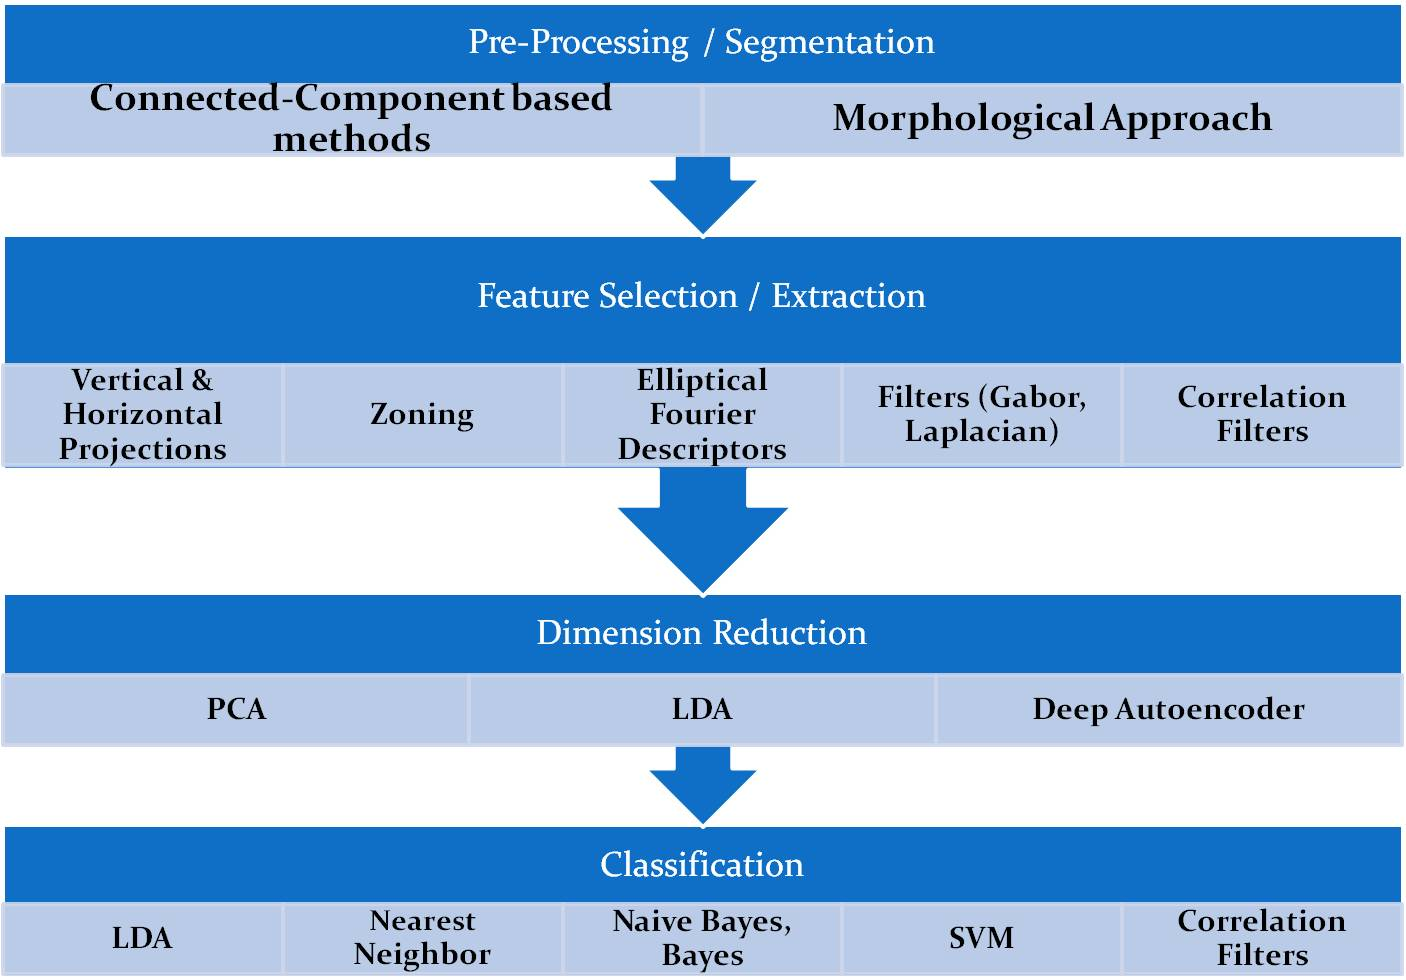
\includegraphics[scale=0.66]{algoOverview.jpg}\\
		%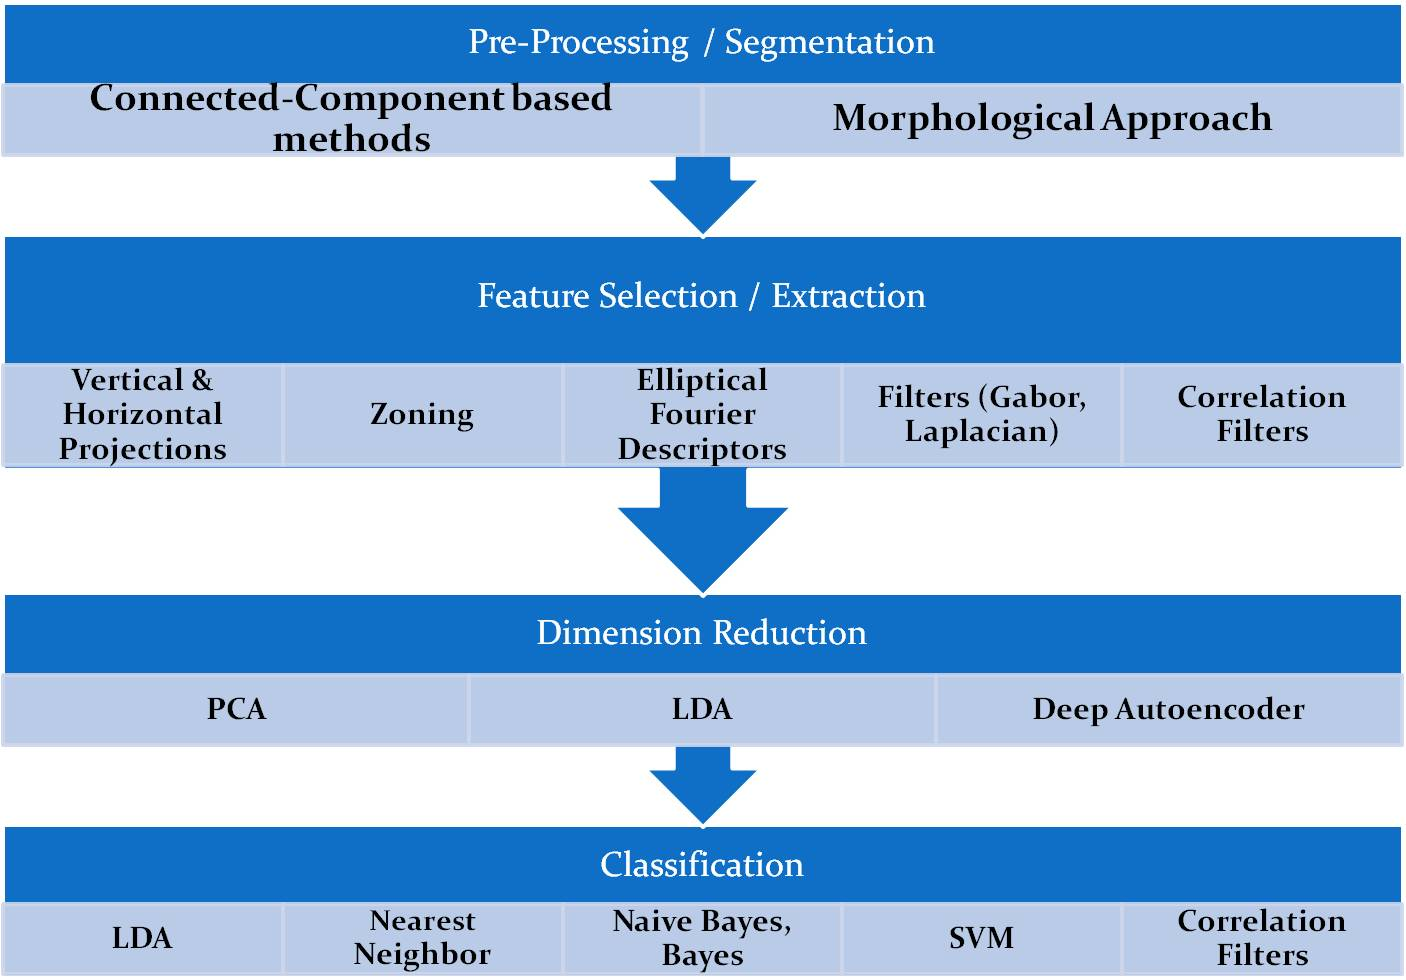
\includegraphics[height=90mm, width=170mm]{algoOverview.jpg}\\
		\caption{Information flow through Core Algorithm}
		\label{fig:algoOverview}
	\end{figure}
As can be seen, we broke up our core algorithm into four main components: Pre-Processing / Segmentation,
Feature Selection / Extraction, Dimension Reduction and Classification. This approach had been used by other teams
also implementing OCR previously \cite{tai, zhidong, sonia}, and we decided to use it based on its simplicity and modularity.\\





\subsection{Principal Considerations}
Due to the nature of our project, we were constrained by both time (~6 weeks), as well as resources (limited number of approaches
to try, platform specifications). Our core considerations, too, in choosing algorithms were:\\

\paragraph{\textit{Simple to implement}} Given our short time frame, we were looking for algorithms that would be simple to implement, and
quick to debug. Simple algorithms would also there was a greater chance of successfully porting it over from MATLAB to Java to C,
or in some cases a built in function might already exist.

\paragraph{\textit{Modular}} Our project had been set up to be modular, with different components being able interchangeable. This allowed us
to quickly experiment with different algorithmic components and gauge the accuracy of that model. Naturally, it was much more beneficial if
the algorithm was modular to fit into our development framework.

\paragraph{\textit{Memory Efficient}} The Android platform does not provide large amounts of memory to its applications. Given that we were
also dealing with large bitmaps sometimes, it was crucial to have a memory efficient algorithm to prevent Out of Memory Errors.

\paragraph{\textit{Fast, Minimum Computation}} We wanted our algorithms to run quickly, and efficiently. In the long run, we hoped to scale
up such that we could work on live data.
\paragraph{\textit{Robustness}} We wanted our OCR engine to be robust to noise, and having algorithms that gracefully deal with this would
be a plus.\\

We then used these considerations as a metric in choosing which algorithms to include into our project. As a benchmark, all testing
of the algorithms in this section was done with the same dataset: Numbers 0-9, Binary images of varying font and rotation. Training
was done on 50 samples, and testing was done on 20 samples, of each number. Figure \ref{fig:sampleData} are some examples of the characters from the training dataset.\\
\begin{figure}[h]
		
\includegraphics{sampleData.jpg}\\
		\caption{Sample of Training Dataset used. Binary images of varying font, and rotation.}
		\label{fig:sampleData}
\end{figure}





\subsection{Pre-Processing / Segmentation}
When choosing components, we first decided on Pre-Processing / Segmentation, as it was the initial step before any computation, and would define
the format of the data we would be training on. We initially experimented with connected component based methods \cite{textDetectionSurvey, ohya},
whereby we would be applying local thresholding for binarization, and detecting blobs of similarly textured grayscale as objects. Essentially,
we were using the gray-level difference of shapes and sizes to make a match. We found it worked relatively well, but was susceptible to noise
and illuminating conditions. Subsequently, we tried another approach. This time we implemented a morphological approach \cite{hassan}, essentially
doing edge detection. We would form a weighted grayscale and identify the edges using a morphological gradient operator. Use of dilation and erosion
allowed us to remove salt and pepper noise, as well as form candidate regions for segmentation. We also found that using adaptive thresholding worked
best for the binary edge image. The algorithm became much more robust to noise and orientation, but was still suscpetible to illumniation, as shown
in the picture below. This was chosen as our segmentation algorithm for the project
\begin{figure}[h]
		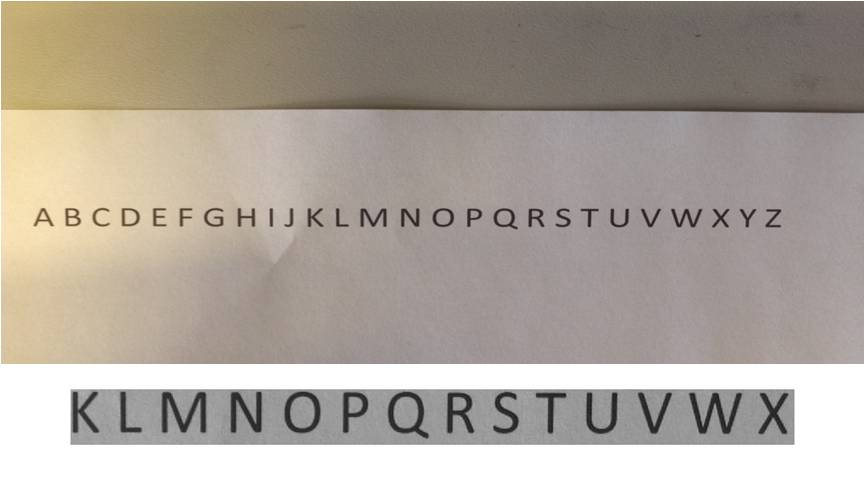
\includegraphics{seg.jpg}\\
		\caption{Morpohlogical Image Segmentation with Strong illumination from left, Above: Image, Below: Detected text}
		\label{fig:seg}
\end{figure}





\subsection{Dimension Reduction}
We next turn our attention to Dimension Reduction. Dimension Reduction tends to have some overlap with feature selection and extraction, but
we decided to seperate it out, to keep our project modular. Dimension Reduction was meant to ensure that the inputs of the feature vector to 
the classifier would be uncorrelated, and that the dimensions would be reduced to a set number. The idea was to decrease computational complexity
of the classification algorithm when training, by using a smaller feature vector that still captured the majority of variance in the dataset.

\subsubsection{Linear Discriminant Analysis}
Linear Discriminant Analysis attempts to model the difference between the classes of data, by taking into account class labels and maximizing the
between-class scatter under the constraint that the within-class scatter is minimized. This results in compact clusters for each class, as far as
possible from each other. To test LDA, we attempted to reconstruct a test image, and measure the mean squared error compared to the original image.
LDA performed well, with almost no reconstruction error.
\subsubsection{Autoencoder}
\begin{figure}[h]
		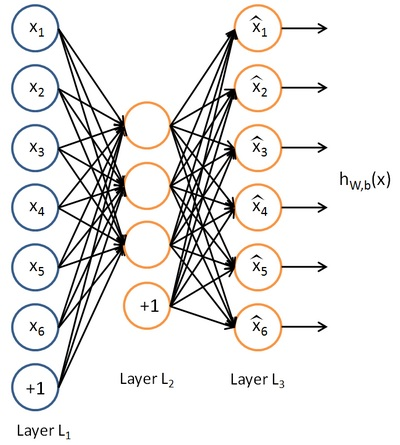
\includegraphics[scale=0.75]{autoencoder.jpg}\\
		\caption{Structure of an autoencoder. Implements Nonlinear PCA by attempting to learn the function $h_{W,b}(x) \approx x$}
		\label{fig:autoencoder}
\end{figure}
Autoencoders are essentially a way of implementing Nonlinear PCA. This is done using a neural network applying backpropagation, where the
hidden layers are used to provide a nonlinear reconstruction. In order to train it, we set the target values to be equal to the inputs, such
that the network attempts to learn an approximation of the identity function, so that the output is similar to the input. By varying the number 
of output nodes (number of nodes in Layer $L_3$,
we can select the number of basis function to use (similar to PCA in how we can choose how many eigenvectors to use). As such, since the number
of hidden units is much less that the input feature vector, Layer $L_1$, the network learns a compressed representation of the input. By imposing
a sparsity constraint on the network, as well as implementing a locally competitive algorithm, could potentially provide us better, more meaningful
representations too. Varying the number of hidden layers also affects the output - multiple sigmoid hidden layers give us our nonlinear representation.
For our project, we tested the autoencoder to see if there was significant benefit using a non-linear approach. We ran the data through a 5-layer 
autoencoder. The representation we got out did not significantly improve beyond PCA.

\subsubsection{Principal Component Analysis}
PCA performed well, and is typically the most basic dimension reduction method to use. For our purposes, we found the reconstruction error to be
~1\% or less, similar to LDA.\\

After our testing, we decided to utilize PCA, due to its simplicity and modularity. It also had inbuilt functions in OpenCV and Matlab, allowing
it to be quickly implemented. The autoencoder might have performed well after additional research (We only tested it thrice), but given the time
constraints, and seeing that it did not bring significant immediate benefit, plus we would essentially have to write the neural network on Android ourselves,
made us decide on using PCA.



\subsection{Feature Selection / Extraction}
In OCR, feature selection is key, and is closely tied to classification. For this section, we will
be decribing some of the features we opted to use \cite{line, jain}. The analysis of their effectiveness is in the Results section.

\subsubsection{Vertical \& Horizontal Projections}
\begin{figure}[!]
		
\includegraphics[scale=0.33]{proj.jpg}\\
		\caption{Diagram showing Vertical and Horizontal Projections}
		\label{fig:proj}
\end{figure}
Figure \ref{fig:proj} shows the vertical and horizontal projection feature. Essentially, it is taking a spatial
histogram of the number of black pixels row by row, and column by column. The feature vector is then the concatenation
of both histogram values. Initial results showed this feature having a \~60\% accuracy on the test dataset mentioned above.
This has the advantage of being simple, and
quick to compute. However, it is susceptible to rotation, as a rotation would shift both histograms by some amount.
In addition, it is also susceptible to illumination. Being in a shadow tends to increase the number of black pixels
shown, and hence will distort the feature vector. In order to test its effectiveness, we varied the number of bins,
to account for some rotation. We also equalized the histogram, and normalized the feature vector. However, these
did not significantly improve the accuracy.\\

\subsubsection{Zoning}
\begin{figure}[!]
		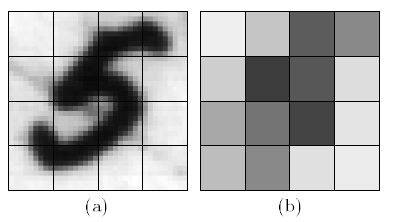
\includegraphics[scale=0.25]{zone.jpg}\\
		\caption{Diagram showing Zoning of Characters: a) Bitmap of Character b) Feature Vector formed}
		\label{fig:zone}
\end{figure}
Figure \ref{fig:zone} Shows how the feature vector is computed during zoning. The rectangle circumscribing the character 
is divided into several overlapping, or nonoverlapping, regions and the densities of black points within these regions are computed
and used as features. Initial results showed this feature also having a \~60\% accuracy on the test dataset mentioned above. Again, this has the advantage of being simple, and
quick to compute. However, it is slightly susceptible to rotation.
In addition, it is also susceptible to illumination. Varying the number of zones, and their overlaps did not. significantly improve the accuracy.\\


\subsubsection{Elliptical Fourier Descriptors}
\begin{figure}[h]
		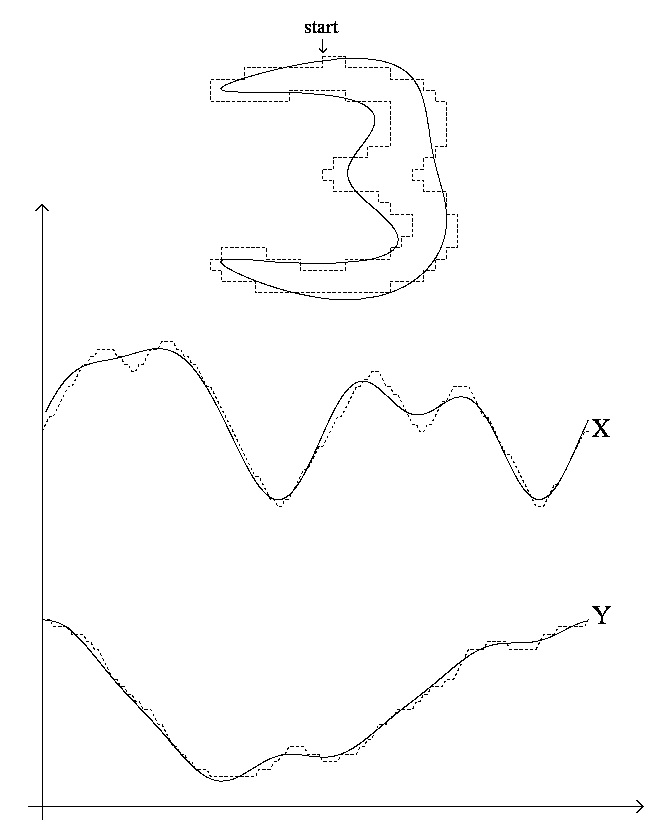
\includegraphics[scale=0.5]{elliptical1.jpg}\\
		\caption{Diagram showing Zoning of Characters}
		\label{fig:elliptical1}
\end{figure}
Figure \ref{fig:elliptical1} shows the construction of the curves from the contours.
The closed outer contour curve of a character is a closed piecewise linear curve that passes through the centers of all the pixels which
are 4-connected to the outside background, and no other pixels. This is because we are only using numbers and upper-case alphabets. Following the
curve, the pixels can be visited in counter-clockwise order, and the curve may visit an edge pixel twice at locations where the object is one-pixel wide.
As such, the contour is made up of line segments, each a straight line between the pixel centers of two 8-connected neighbors. By approximating the
contour curve by a parametric expression, the coefficients of the approximation can be used as features. By following the close contour successively,
a periodic function results, which are well suited to Fourier series expansion. This requires an arbitary stating point to be chosen. To mitigate this,
we calculate the phase shift from the first major axis, and rotate the coefficients to achieve a zero phase shift. For rotational invariant descriptors, the rotation
of the semi-major axis is found and descriptors are rotated once more. Size invariance is achieved by dividing by the magnitude of the semi-major axis.
Elliptical Fourier Descriptors are used to reduce the dimensionality of the feature vector and the extract features made invariant to global deformations
such as translation and rotation.

\begin{figure}[h]
		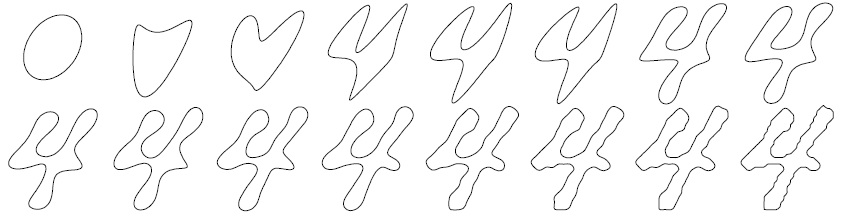
\includegraphics[scale=0.75]{elliptical.jpg}\\
		\caption{Character '4' reconstructed by elliptic Fourier descriptors of orders up to 1, 2, ... 10; 15, 20, 30, 40,  50, and 100 respectively}
		\label{fig:elliptical}
\end{figure}
Figure \ref{fig:elliptical1} shows the reconstruction of the character using elliptic fourier descriptors. As additional terms are added, the accuracy of
the curve increases. This feature take longer to compute, however, it is both rotational and size invariant. We are also able to choose the number
of 'harmonics' we would like to use, therefore giving us flexibility in choosing our feature vector. The initial implementation of the elliptical fourier
descriptor was written by us, however, later version referenced online sources.

\subsubsection{Filter (Gabor, Laplacian)}
We utilized both the Laplacian and Gabor filters in our filter bank. Both filters are useful as spatial edge detectors, and produced
good results when we initialized our Gabor filter bank with different frequencies and orientations. As we learned in the homework, this produced
good features for discrimination. However, our feature vector was extremely large, and slow to compute due to the numerous computations and convolutions.

\subsubsection{Correlation Filters}
The correlation filters will be elaborated in greater detail in the results section.



\subsection{Classification}
In choosing our classification method, we decided to take two different approaches to implement the OCR engine. We wanted
to try both the feature matching and template matching approaches, and as such chose to use SVMs and Correlation Filters in the final product.

\subsubsection{Linear Discriminant Analysis}
LDA performed well in classification, with an accuracy of \~95\%. This is probably as the disciminatory information was in the mean of the data.
However, it did not bear itself well to implementation on the Android platform, and produced a hard bound of at most number of classes -1 feature
projections. When scaling up to the full alphabet, it did not seem likely continue to be modular on the Android platform. As such, we decided not
to proceed with using LDA.

\subsubsection{Nearest Neighbor}
Nearest neighbor is a simple classifier that is based on the nearest-neighbor approach. For classification, one simply finds the N-dimensional 
feature space the closest character from the trainng set to an character being classified. if the neighbor is nearby, it is likely to be similar to 
the character being classified and so can be grouped as such. It is simple to implement, can be generalized to k-means, and worked reasonably 
well for small datasets (\~85\% accuracy). However, when increasing the number of classes, as well as the necessary training data, we found 
that accuracy decreased significantly. Choosing parameters was also tricky, in that it seemed sensitive to the presence of irrelevant parameters.
In addition, the training set is retained in its entirety as a description of the character distribution,
and with our current memory constraints on Android, it did not seem particularly fruitful. 

\subsubsection{Naive Bayes}
The Naive Bayes classifier was fast to train and evaluate, and seemed to perform well quickly on small datasets (5 characters, 50 training samples),
with an accuracy of \~95\%. However, when scaling up the number of classes the algorithm did not seem to be able to solve the harder classification
problems with the same amount of accuracy. Naturally, the algorithm assumes that the features are independent, which is probably not true given our
data. As such, we decided to not to pursue Naive Bayes in our implementation.

\subsubsection{Support Vector Machine}
Support Vector Machines are powerful non-linear classifier that gave us great potential for an OCR engine, given that we could
have good features. While they were slow to train, they consistent produced good results (\~99\% accuracy with 10 classes). In addition,
by increasing the dimensionality of the data, the characters get easier to separate, allowing it to solve classification problems with
arbitarry complexity. Using the dot product, and the model's support vectors (there is no need to store all the points in an SVM), with biases,
we thought it would be possible to move a trained SVM onto the android platform, with less of a memory footprint than expected. As such, it seemed
that given the great potential, the only risk would be bad features and a long training schedule. We later mitigated this by training our
SVMs on the ECE Servers over command line - with 8 Cores running lots of RAM, we could train our entire dataset of 25200 characters in 2 hours.

\subsubsection{Correlation Filters}
The correlation filters will be elaborated in greater detail in the results section.

\section{Results}

\subsection{Data}
As shown earlier, Figure \ref{fig:sampleData} is an example of some of the data we trained and tested with.
The training data consisted of 700 binary images for each character, with of different rotation and fonts.
The training data is a processed data set using our segmentation algorithm. This helps to keep our
training and testing data as realistic as possible. In addition, we also used images captures from the
tablet to perform periodic checks that our OCR was working properly.

\subsection{SVM}

\subsubsection{Training}
AS mentioned above, we utilized the different features to come up with a composite feature vector.
We took care to ensure that there was invariance with respect to rotation, illumination and size,
and that the algorithm did not take too long to run. We also experimented with Hough Transforms,
but it did not seem to suit our data, as it was projecting obvious lines. Skeletonising the characters
yielded little benefit if at all. We also experimented with using some expert-driven features \cite{frey}. We 
found this method from an online journal article about letter classification that 
spoke of a set of sixteen numerical attributes that when used to 
classify the 26 characters of the alphabet would completely separate the classes. 
These sixteen attributes were extracted after a pixel-by-pixel scan of the character. 
Included in these sixteen attributes are:\\
1. The horizontal position, counting pixels from the left edge of the image, of the center of the smallest 	rectangular box that can be drawn with all "on" pixels inside the box.\\
2. The vertical position, counting pixels from the bottom, of the above box.\\
3. The width, in pixels, of the box.\\
4. The height, in pixels, of the box.\\
5. The total number of "on" pixels in the character image.\\
6. The mean horizontal position of all "on" pixels relative to the center of the box and divided by the 	width of the box. This feature has a negative value if the image is "leftheavy" as would be the 	case for the letter L.\\
7. The mean vertical position of all "on" pixels relative to the center of the box and divided by the 	height of the box.\\
8. The mean squared value of the horizontal pixel distances as measured in 6 above. This attribute will 	have a higher value for images whose pixels are more widely separated in the horizontal 	direction as would be the case for the letters W or M.\\
9. The mean squared value of the vertical pixel distances as measured in 7 above.\\
10. The mean product of the horizontal and vertical distances for each "on" pixel as measured in 6 and 	7 above. This attribute has a positive value for diagonal lines that run from bottom left to top 	right and a negative value for diagonal lines from top left to bottom right.\\
11. The mean value of the squared horizontal distance times the vertical distance for each "on" pixel. 	This measures the correlation of the horizontal variance with the vertical position.\\
12. The mean value of the squared vertical distance times the horizontal distance for each "on" pixel. 	This measures the correlation of the vertical variance with the horizontal position.\\
13. The mean number of edges (an "on" pixel immediately to the right of either an "off" pixel or the 	image boundary) encountered when making systematic scans from left to right at all vertical 	positions within the box. This measure distinguishes between letters like "W" or "M" and letters 	like 'T' or "L."\\
14. The sum of the vertical positions of edges encountered as measured in 13 above. This feature will 	give a higher value if there are more edges at the top of the box, as in the letter "Y."\\
15. The mean number of edges (an "on" pixel immediately above either an "off" pixel or the image 	boundary) encountered when making systematic scans of the image from bottom to top over all 	horizontal positions within the box.\\
16. The sum of horizontal positions of edges encountered as measured in 15 above
The best accuracy that was found using the sixteen attribute set as the feature selector was 72.45\%, 
which isn't nearly as accurate as the other combinations of features. Because of these slow processes, 
training the images takes a very long time along the lines of four to five hours. While training only needs 
to be done once in order to use the Support Vector Machine, the testing also is not quick at all and takes 
awhile to calculate and compare the images' attributes making this process a very slow one.  
One solution we considered is removing and adjusting some of the attributes as to speed up the 
process while still maintaining the accuracy of this method.  Since attributes thirteen through 
sixteen were the main contributors to the speed issue, we chose to remove them and try to see if 
the accuracy would still remain the same.  When testing on the same test data as the original data, 
the twelve attribute set accuracy was greatly reduced from the set using all sixteen attributes.  
The accuracy we got from the twelve attribute set was 48.15\%.  
These results may have occurred because of many reasons.  
The reason for errors when using the sixteen attribute set seem to be 
from rotation, illumination, and the various fonts used in the simulation.  
The rotation will affect many of the attributes such as the edges and the horizontal 
and vertical positions which will throw off the strength of the correlation between each 
character.  With the illumination involved in the image, the binary interpretation of the 
image would definitely change the image because illumination would change multiple areas that 
were “off” pixels into “on” pixels. \\

Finally, we did further analysis on using differnt combinations, as well as differnt feature vector length, 
of the previous elaborated features, e.g. fourier descriptors etc. 
Training was sped up using the ECE servers. (8 cores were able to train 25200 images in 2 hours).

\subsubsection{Results}
\begin{figure}[h]
		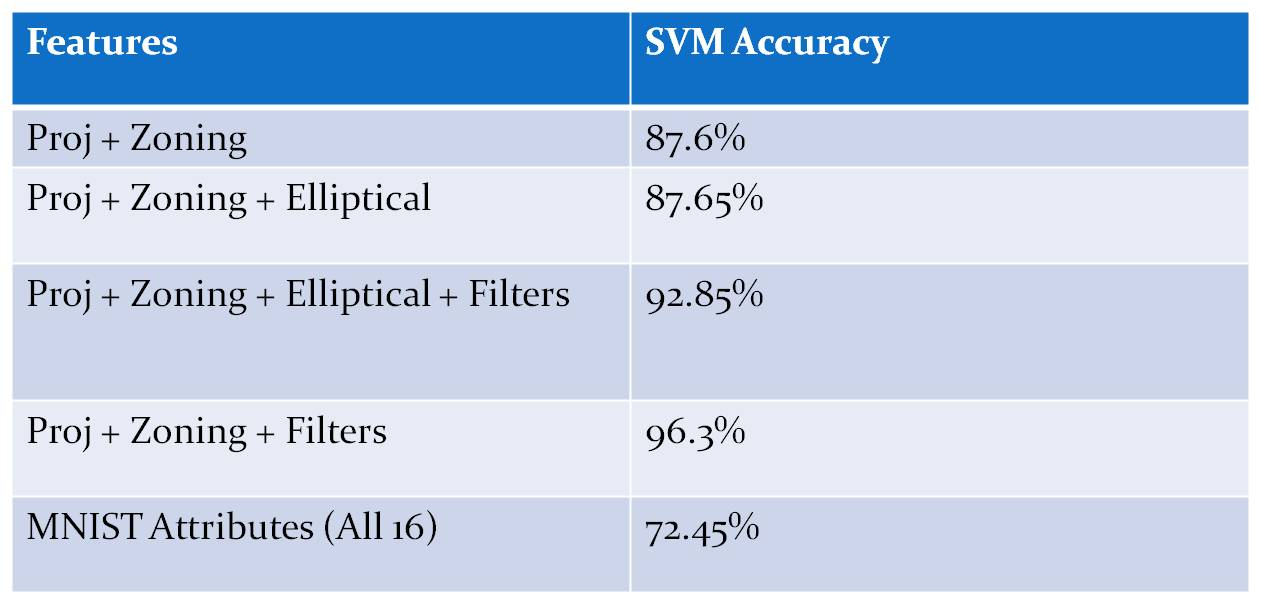
\includegraphics[scale=0.80]{svmResults.jpg}\\
		\caption{Figure showing the accuracy using different features for our SVM}
		\label{fig:svmresults}
\end{figure}
Figure \ref{fig:svmresults} shows that the filters together with zoning seem to be most effective.
In this case, we had used a filterbank of 6 different orientations of Gabor filters,
and combined with zoning, seems to have given the best accruacy at 96.3\%. This is probably due
to the gabor filter's effectiveness in detecing the differnt edges. Furthermore, research has also
shown that typically the sparse codes basis for natural images, tend to have gabor like features.
In this sense, our results confirm their findings. However, it is very computationally expensive
to run the characters through the filterbank and our processing time suffers for it.


\subsection{Correlation Filters}
Another optical character recognition method we used was correlation filters. 
Unlike SVMs, correlation filters use templates based on far fewer training 
images to compare to the input image. While less robust than SVMs, we found 
that the correlation filters were much easier and quicker to train at the 
expense of requiring one filter per letter, font, and greater than \~5 degrees 
of rotation. Because we initially focused on recognizing only capital letters 
in one font, however, the results showed high accuracy, often categorizing all 
26 input characters correctly.\\
All of the filters were first coded in Matlab for testing, and only once the most 
steadily accurate filtering algorithm was confirmed did we attempt to convert the 
code into a language able to be handled by the Android tablet. Unfortunately, the 
code conversion was far more complicated than we anticipated, and only the 
simplified versions of the correlation filters were able to be implemented. We did, 
however, use the Android server/client system to send images through the Matlab 
code to ensure the filters would work if the tablet could run the code.

\subsubsection{Simple Correlation}

\begin{figure}[h]
		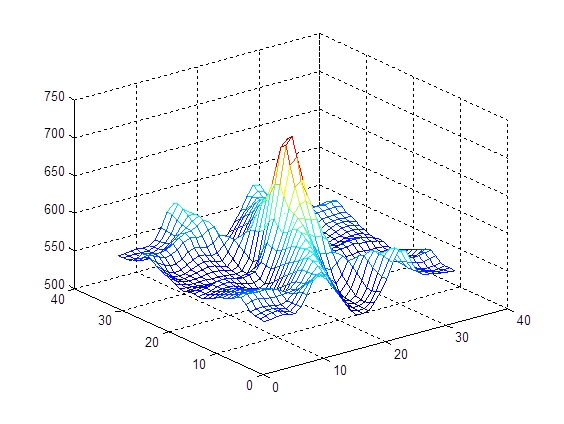
\includegraphics[scale=0.80]{corr.jpg}\\
		\caption{Simple Correlation Energy Plane between input 'A' and 'A' filter.}
		\label{fig:corr}
\end{figure}


\begin{equation}
\label{eqn332}
Correlation = ifft2(fft2(input).*conj(fft2(filter)));
\end{equation}

The first correlation filter we implemented worked off a 
single template image ('filter', in \eqref{eqn332})
for the correlation equation (\eqref{eqn332} documents the Matlab 
code used). While we initially had some trouble generating the 
appropriate figures, we soon learned how similar the training 
and testing images needed to be in order to achieve pleasing results 
(see figure \ref{fig:corr} for an example). Once the code was modified, 
the simple correlation filters showed an average of an 89% success rate 
across over 100 tested characters, though our final testing set for the
demonstration yielded a 0\% success rate across 26 
capital-letter inputs. While just under half of the initial testing 
characters were derived from the same images used to generate the training 
data, we did not detect a noticeable difference across testing sets. Further, 
the tested characters were passed through different filters than the training 
characters to provide noise and rotation in order to ensure variance between 
sets. As our final testing set provided noisier inputs to thoroughly test the 
robustness of the various OCR methods, we were not surprised to find that the 
simple correlation filter had such a low accuracy.\\
\\
The same training and testing data was used for all of the following 
correlation filter algorithms. While we would have liked to test on a 
larger number of inputs, the illumination greatly affected the accuracy 
of the filters, leaving us with far less usable images than desired. 
Though more rigorous testing may result in slightly lower success rates, 
we are confident that the difference would not contradict the general 
overview of our results. Further, because 26 filters could be generated 
in a matter of seconds, tweaking the noise filters before correlation 
allowed us to increase categorization success quickly depending on the 
location in which the input image was captured.

\subsubsection{Equal Correlation Peak - Synthetic Discriminant Function}

\begin{figure}[h]
		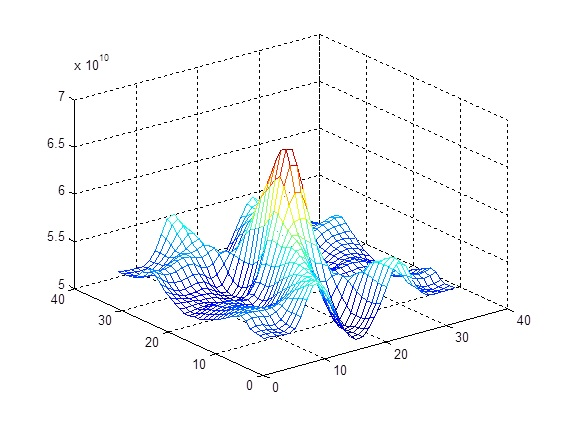
\includegraphics[scale=0.80]{corr1.jpg}\\
		\caption{ ECP-SDF Correlation Energy Plane between input ‘A’ and ‘A’ filter}
		\label{fig:corr1}
\end{figure}

\begin{equation}
\label{eqn333}
H = X(X+X)^{-1} u
\end{equation}

The next filter we coded and tested was an ECP-SDF. The main difference between
this filter - and the two following - and the simple correlation filter is that
these filter algorithms allow more than one training image 
to generate the template for correlation. In order to accomplish this, 
the Fourier transform of 'filter' in \eqref{eqn332} is replaced with \textbf{H}, an 
aggregate vector of the training images in the frequency domain \textbf{(X)}, as 
described in \eqref{eqn333} Further, this and the following filters allow 
training images to be weighted via u, a one-dimensional vector containing 
1s for a positive correlation and -1s for the opposite. While this would 
mainly be used to differentiate similar characters from one another, i.e. 
'E' and 'F', we found that too many training images corrupted the filters, 
preventing them from working as intended.\\

Surprisingly, despite the seeming increase in robustness of the 
pre-correlation algorithm, the ECP-SDF performed more poorly than 
the simple correlation filter, with an average accuracy of around 
70\% over the initial testing set. Despite the large decrease in successful 
categorizations in the testing sets, the correlation energy planes are 
hardly distinguishable from those of the simple correlation filters (figure \ref{fig:corr1}), 
and the ECP-SDF algorithm worked significantly better than the simple filters over
the final demonstration inputs, achieving a 61.5\% categorization accuracy there.
\subsubsection{Minimum Average Correlation Energy Filter}

\begin{figure}[h]
		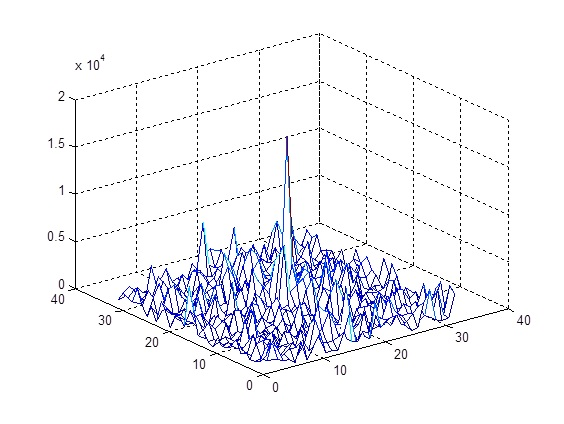
\includegraphics[scale=0.80]{corr2.jpg}\\
		\caption{MACE Filter Correlation Energy Plane between input ‘B’ and ‘B’ filter.}
		\label{fig:corr2}
\end{figure}

\begin{equation}
\label{eqn3341}
H = D^{-1}X(X+D^{-1}X)^{-1} u
\end{equation}

\begin{equation}
\label{eqn3342}
D_{i}(k, k) = |X_{i}(k)|^{2}
\end{equation}

The MACE filter alters the equation for H \eqref{eqn3341} by introducing D \eqref{eqn3342}, 
a diagonal matrix of the power spectrum of the training images. In Matlab, this was done 
by averaging the magnitude square of the training images in the frequency domain.

As seen in figure \ref{fig:corr2}, the MACE filter correlation energy plane differs 
dramatically from those of the previous two correlation filters. The more 
pronounced peak yields far better results as well, achieving an average accuracy 
of 100\% over the initial testing sets, and 88.5\% categorization accuracy over the 
final demonstration set.

Because of the success rate, we selected the MACE filter for 
the majority of the debugging and testing of the various PSR 
algorithms (see PSR Section). This was mostly done before the 
final demonstration set was generated, though, which partially 
helps to explain our decision.

\subsubsection{Optimal Trade-Off Synthetic Discriminant Function}
\begin{figure}[h]
		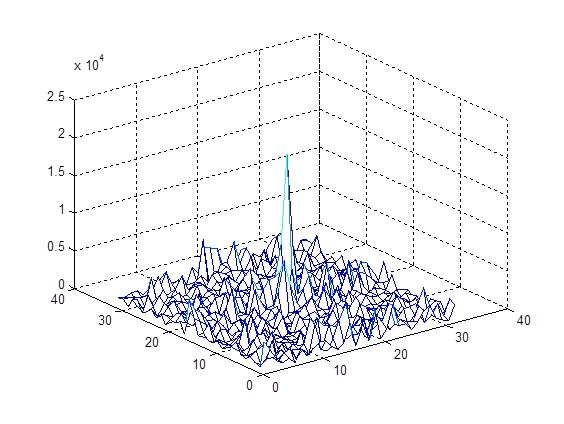
\includegraphics[scale=0.80]{corr3.jpg}\\
		\caption{OTSDF Correlation Energy Plan between input ‘B’ and ‘B’ filter.}
		\label{fig:corr3}
\end{figure}
The final filter we coded and tested was the OTSDF. 
While very similar to the MACE filter (see figure \ref{fig:corr3}), 
the OTSDF alters \textbf{D} to handle noise \eqref{eqn3351}. In the equation, $\alpha$ 
can be selected based on the amount of noise to train for, and $\beta$ simply 
depends on $\alpha$ \eqref{eqn3352}. Though we initially tested with $\alpha = 0.99$, we 
found that $\alpha = 0.75$ accounted for our input better, especially for the final 
demonstration data set.

\begin{equation}
\label{eqn3351}
D_{new} = \alpha D_{MACE} + \beta I
\end{equation}

\begin{equation}
\label{eqn3352}
\beta = \sqrt{(1 - \alpha^{2}}
\end{equation}

In testing, the OTSDF averaged 100\% accuracy with the same testing data sets as the other three correlation filters, but due to pre-processing, the value of $\alpha$ did not affect results. However, during our preparation for the demonstration, we found that the OTSDF, while more accurate than the MACE filter, repeatedly categorized 'F' as 'E'. This was when we learned of the usefulness of the change to \textbf{D}; blurring the training images to add noise after pre-processing, along with an adjusted $\alpha$, allowed for 100\% correct categorization over the final demonstration inputs. \\
Because of the accuracy and superior robustness of the OTSDF, while we were unable to convert the Matlab code entirely to the Android application, we realize this is the most promising of the correlation filters.

\subsubsection{Peak-Sidelobe Ratio}
As a way of measuring the success of a correlation (\textbf{C}), we computed the PSR of the correlation energy planes. This allowed us to quickly tell which filter matched each input best, allowing the categorization of each character to process smoothly. Initially, we calculated a simplified version of the PSR in Matlab \eqref{eqn336} to compare the various correlation filters. While this computation worked for debugging, a more accurate algorithm was necessary.

\begin{equation}
\label{eqn336}
PSR_{simple} = (max(C) - mean(C)) / std(C);
\end{equation}

In order to more properly calculate the PSR, by definition, we needed to take the mean and standard deviation of the sidelobe of the correlation energy plane. To do so, we essentially masked a 5x5 area of the correlation centered on the maximum value, and used the rest of the values for the sidelobe. While this was not necessarily the best way to compute the PSR, we saw a noticeable difference in our results (figure \ref{fig:alexTable}). Unfortunately, the masking process did not convert to the Android easily, but we found that the simplified PSR worked to a reasonable extent, at least allowing us to compare the correlation filter method of OCR to the other processes.

\begin{figure}[!]
		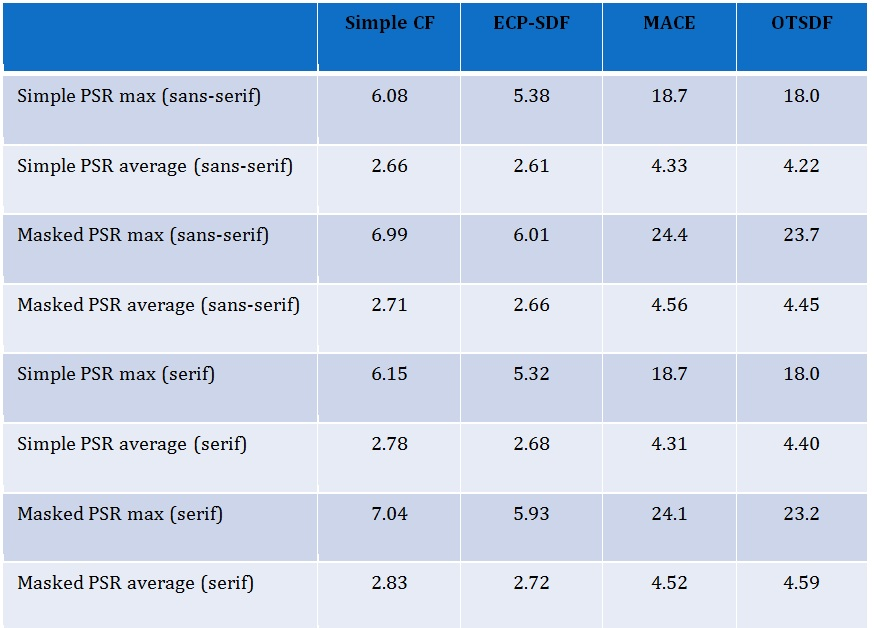
\includegraphics[scale=0.66]{alexTable.jpg}\\
		\caption{Simplified and masked PSR data for each correlation filter across serif and sans-serif testing sets.}
		\label{fig:alexTable}
\end{figure}

\newpage
\section{Implementation}
During the implementation phase, we encounter several challenges due to integration issues,
as well as in our developmental workflow. We constantly iterated and tried new approaches.
Our three main approaches that worked to product a functional OCR are outlined below.

\subsubsection{Native Android App - OpenCV}
We initially attempted to implement a native android application, using the Java Native Interface
to run OpenCV C++ code. However, we were quickly bogged down by dependency and programming environmental
issues. After a painstaking week of debugging, we realized that due to the android platform, we would
not be able to run both JavaCV and native OpenCV in the same application - an error was thrown about
a duplicate in the .apk file. \\
Nevertheless, we were able to get a quick prototype up and running.
The code can be found in the 18551\_Prototype android project. We were able to get a touch-based
selection box working. As a prototype, we also managed to linked tesseract - Google's Open Source OCR Engine - 
to our application giving us decent OCR capabilities. These were done through different Views and Touchevents.\\

However, as mentioned there were integration issues,
and we decided to move the project fully onto JavaCV, rationale being that we had only one member - James - 
that was knowledgeable about C/C++, and in this way more team members could contribute.

\subsubsection{Android App - JavaCV}
\begin{figure}[h]
	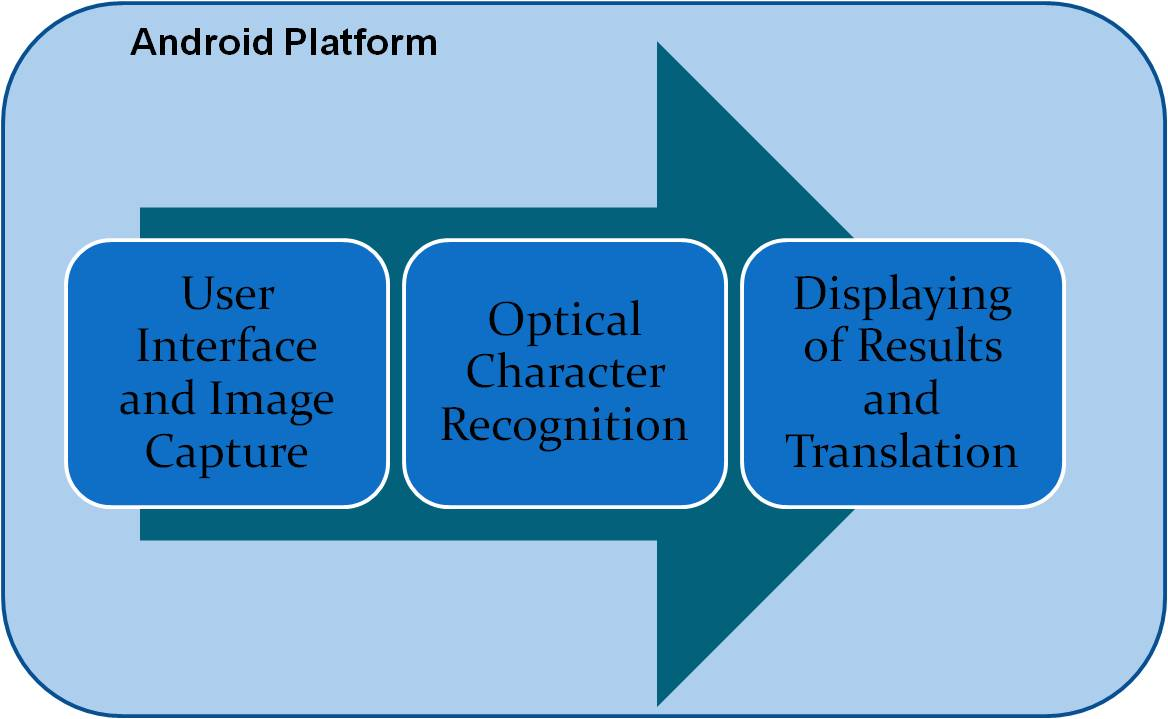
\includegraphics[scale=0.75]{androidFramework.jpg}\\
	\caption{Framework for Android JavaCV App}
	\label{fig:androidFramework}
\end{figure}
Figure \ref{fig:androidFramework}  shows our framework for the Android JavaCV App. After the initial integration issues
with the native Android App, we transitioned over to a pure JavaCV application. As shown, everything occurs
on the Android platform itself. Naturally, however, this had its drawbacks, namely being cumbersome to iteratively
develop on. Loading of android application (apk) files were slow - it could take up to 30 seconds to compile, upload
and install the application on the device. The Android platform itself also had a limited amount of memory, and
was unable to handle more than 3 large bitmaps (i.e. 1592 x 2944 size) bitmaps at a time, which slowed our debugging
process. Processing speed was also much slower than in Matlab on a laptop - early implementations took ~14 seconds to
pre-process the image. Finally, little documentation for Java OpenCV functions existed, slowing progress. Due to these
conditions, and the fact that one of our team members was only fluent in Matlab, spurred us to create another framework
for debugging and development. The code can be found in the 18551\_Project android project.

\subsubsection{Android Client Server Model}
\begin{figure}[h]
	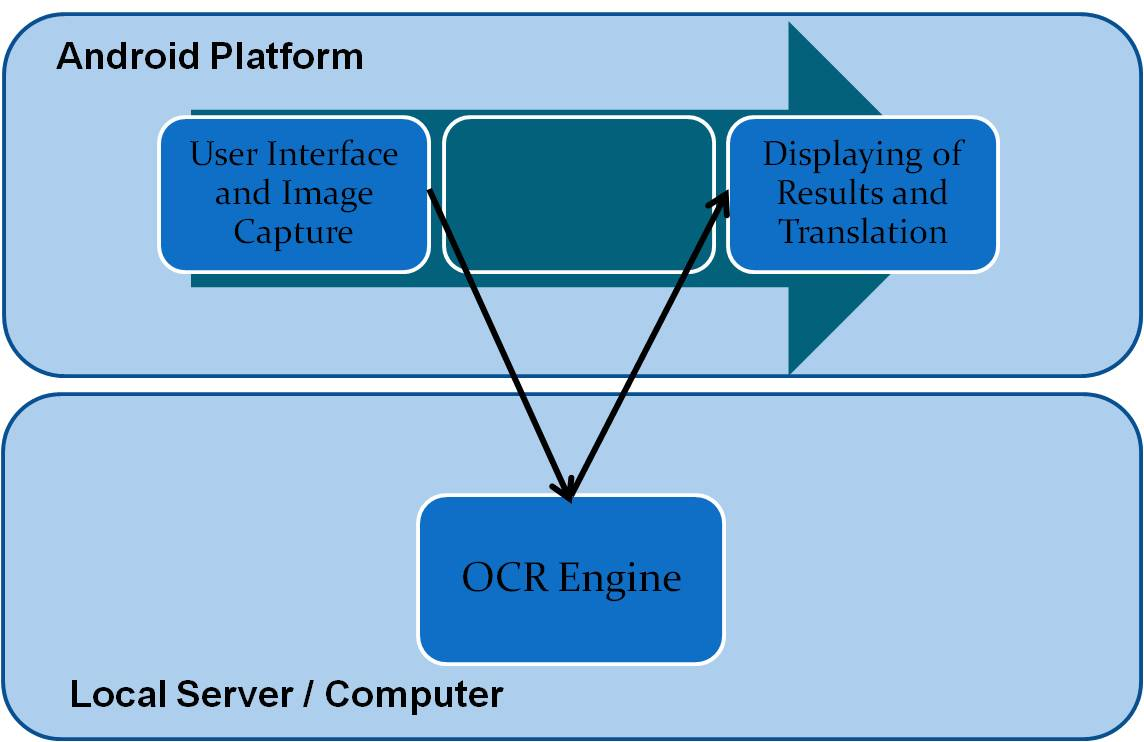
\includegraphics[scale=0.75]{androidCSFramework.jpg}\\
	\caption{Framework for Android Client Server Model}
	\label{fig:androidCSFramework}
\end{figure}
Figure \ref{fig:androidCSFramework} shows our framework for the Android Client Server Model. This was done so that our team could test
and iterate much quicker, in Matlab, while still interfacing with the Android platform, and dealing with the noise
of that system. As shown, the Matlab server is now on our local computer, allowing us to quickly different algorithms
and test it in the real world. Training our SVM is also much easier on our computer. Essentially, the Adroid device
communicates with a local Java Server, which then presents the data to our Matlab Server OCR enginer. After computation,
the Java server then pushes the data back to the Android device for it to update its display. The code can be found 
in the 18551\_Project\_Client and 18551\_Project\_Server android projects.

\subsubsection{Translation}
Originally, we also wanted to implement a 
post-processing method to convert the correct 
ASCII output to another language, allowing for a 
more convenient, directed application. We planned to 
use the Google Translation API for the translation, but 
we came across too many issues with the code. The limited 
documentation for our intended use, along with server connection 
problems, eventually took up too much time of the project. 
Therefore, instead of focusing on solidifying this part of our 
original project idea, we chose to spend our efforts on developing 
the rest of the project, mainly the OCR methods.

\subsection{Optimization}
During our development, we were conscious to continue optimizing for the efficiency. Using these optimizations, were able
to decrease our time for computation from \~16s to \~5s (given 8 characters).
\paragraph{Memory} Due to memory constraints, we 
made sure to allocate efficiently, and utilize the garbage collector as much as possible, to reduce our memory footprint.
\paragraph{Multi-Threaded} Another optimization we used implementing a multi-threaded processing thread to ensure that program could continue
to run smoothly, even under heavy processing load. 
\paragraph{Bitmap formatting} We also optimized the formatting of the bitmaps. Most of our computation was done on single channel binary
images, thus saving processing time (as opposed to using 4-channel RGBA). We also experimented with different ways of loading
the bitmaps, or even saving it to the sdcard, when not in use (to conserve memory). Using this method, we were able to compute quickly,
and display the results (We are actually overlaying the binary image results over the RGBA, making it seems as if we calculated using RGBA values).
\paragraph{Downsampling} Downsampling provided great benefits too. By downsampling, we were able to reduce our computational complexity
greatly. In addition, this also had the added benefit of removing noise to a certain extent. For global features (ie rotating the image to correct
position), we implemented downsampling to good effect.
\paragraph{Faster Search} For the correlation filter, we quickly segmented and scaled the images to the size of their correlation filters. Thus 
our correlation filters did not have search the entire image for the character, merely searching our segmented characters, greatly saving time. 
This is especially so considering the size of an image (1592 x 2944) vs a character (128 x 128) multiplied by the number of classes 
(typically 36 - Numbers and Uppercase Alphabet), is large.
\section{Final Product Demo}
\begin{figure}[h]
	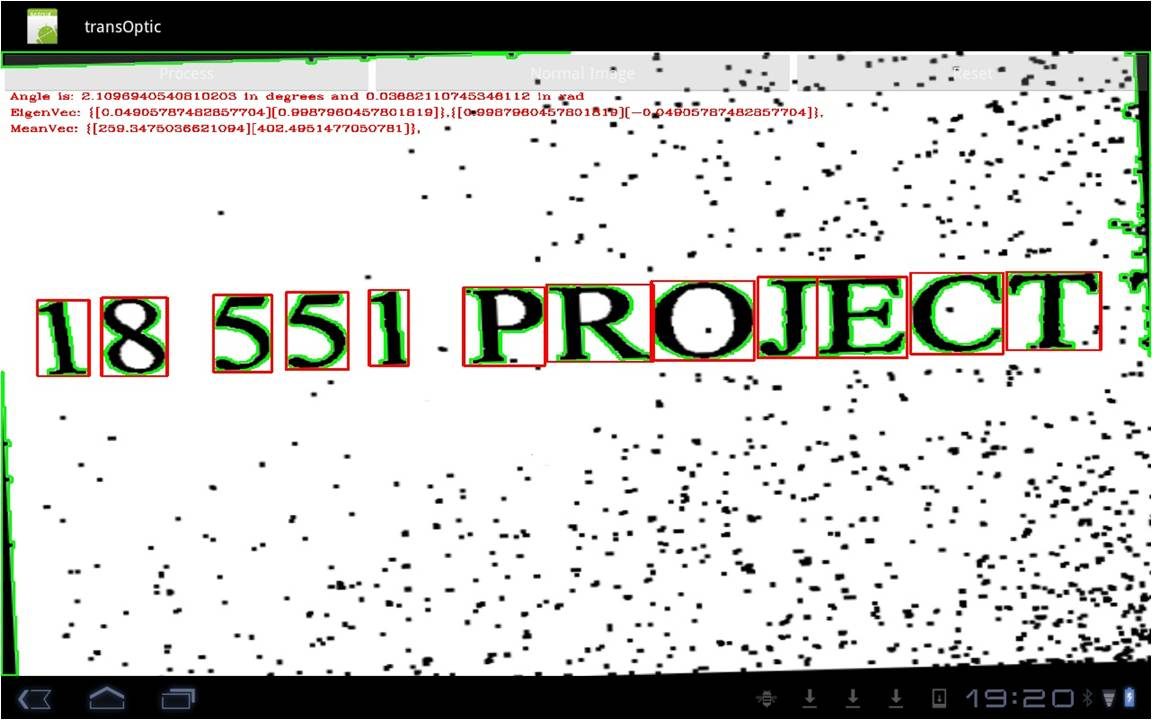
\includegraphics[scale=0.75]{demo.jpg}\\
	\caption{Final Output of Android JavaCV App}
	\label{fig:demo}
\end{figure}

Our final product included two applications, one being the JavaCV version,
and the other being the Android Client-Server Model. 

\paragraph{JavaCV version} Demo was able to rotate and segment characters
using the Android platform and JavaCV. It then implemented our correlation template
matching for deduce the characters on screen.

\paragraph{Android Client Server} Demo was running using a trained SVM on
the local computer. As shown in class, and during the demonstration, the SVM
was able to classify text correctly, with noise, and rotation.



\newpage
\section{Conclusion}

\subsubsection{Future Work}

\paragraph{Neural Networks} We would hope to explore using neural networks
more. Ideally, we hope to develop on our research with Gabor filters and experiment
with Boltzmann machines to gradually develop a convolution neural network \cite{yannle, yannle2}.
We plan to continue development, with the repository continuing to be
updated on github.

\paragraph{Character Location} One benefit of 
correlation filters we were unable to test is their 
ability to provide the locations of the categorizations. 
This would be done by correlating the input data with the 
filters in the position domain, essentially allowing the filter 
to iterate across a larger image. Ideally, the results would 
yield a correlation energy plane with peaks signifying the location 
and class of each character, removing the need for the 
segmentation portion of pre-processing.

\paragraph{Correlation Filter Optimizations} Additionally, 
there is still much that can be done to optimize our 
correlation filters. We would like to improve our PSR 
algorithm to compute a smaller sidelobe and test various 
sizes to find the most accurate and robust area around the 
peak. Further, we can still optimize the correlation filter 
categorization process as a whole, generating a larger number 
of filters with training data to account for more characters, 
different fonts and rotation, and better noise handling. Because 
the correlation filters did not take long to train, we anticipate 
that adding fonts would not too greatly increase the time required 
to generate the filters; however, it would be interesting to compare 
the time and power necessary for the correlation filters to approach 
the versatility of other OCR methods.

\paragraph{Translation} While we were unable to get the 
translation portion of the project completed, it remains 
a critical step in our original project idea. As such, 
we would intend to resolve the issues we ran into previously 
and make the translation a working part of the post-processing section.


\subsubsection{Semester Schedule \& Work Distribution}
\begin{figure}[!]
		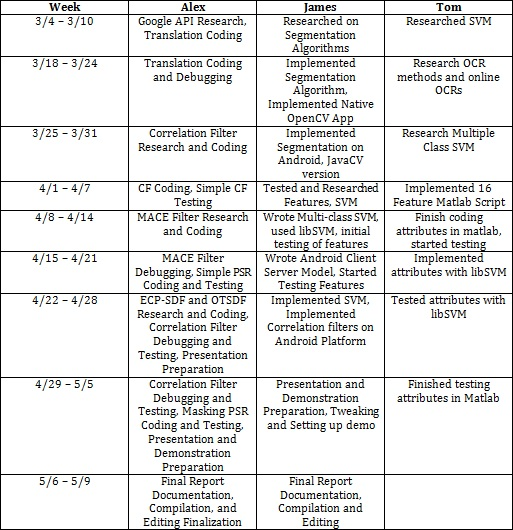
\includegraphics[scale=1.00]{schedule.jpg}\\
		\caption{Schedule of work done over semester}
		\label{fig:sch}
\end{figure}

\begin{figure}[!]
		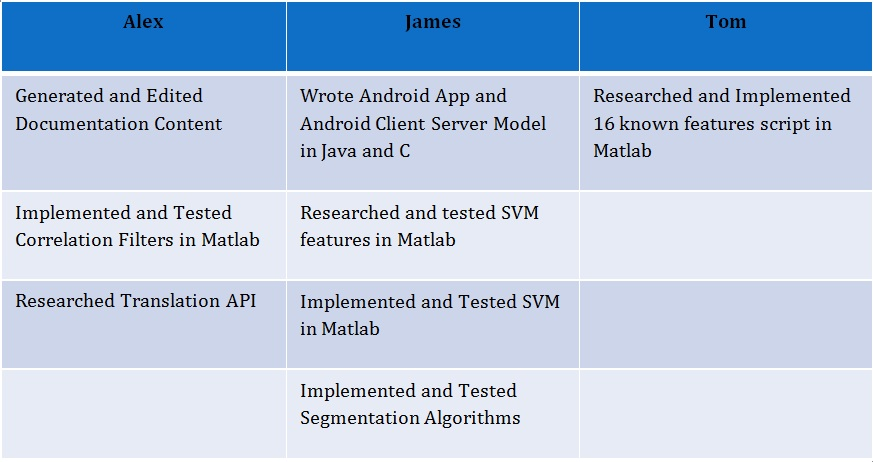
\includegraphics[scale=0.75]{work.jpg}\\
		\caption{Final Distribution of Work and Responsibilities}
		\label{fig:work}
\end{figure}
\newpage
\section{Credits}
{\em
	Our project team would like to thank the following people for their support and guidance.
	
	\paragraph{Professor Tom Sullivan} for teaching and conducting the course
	\paragraph{Professor Marios Savvides} for your advice, guidance and encouragement on our project
	\paragraph{Point TA Yogesh} for meeting with us on weekends, and helping us debug and understand the theory
	\paragraph{Lab TAs} for helping us with all our Android questions
	\paragraph{Everyone in CIC 1308} for giving us great ideas to run with
	\paragraph{Classmates} for having awesome projects and challenging us to do as great a job
}

\newpage
\begin{thebibliography}{99}

\bibitem{class}
  Savvides, Marios
  \textit{18-551 Class Notes}

\bibitem{jeffBier}
  Jeff Bier,
  \textit{Computer Vision In Mobile Devices: The Next Killer App?}
  http://www.bdti.com/MyBDTI/pubs/201104\_compvision.pdf
  
\bibitem{satadal}
  Satadal Saha, Subhadip Basu, Mita Nasipuri and Dipak Kr. Basu,
  \textit{A Hough Transform based Technique for Text Segmentation}
  
\bibitem{xiaoqing}
  Xiaoqing Liu and Jagath Samarabandu,
  \textit{Multiscale Edge-based Text Extraction from Complex Images}
  
\bibitem{basil}
  Basil As-Sadhan, Ziad Al Bawab, Ammar El Seed, Mohamed Noamany,
  \textit{Comparative evaluation of different classifiers for robust distorted-character recognition}
  
\bibitem{tai}
  Tai-Ning Yang, Sheng-De Wang,
  \textit{A rotation invariant printed Chinese character recognition system}
  
\bibitem{zhidong}
  Zhidong Lu, Issam Bazzi, Andras Kornai, John Makhoul,Premkumar Natarajan, and Richard Schwartz
  \textit{A Robust, Language-Independent OCR System}
  
\bibitem{sadhya}
  Sandhya Arora, Debotosh Bhattacharjee, Mita Nasipuri, 
  \textit{Combining Multiple Feature Extraction Techniques for Handwritten Devnagari Character Recognition}
  
\bibitem{tess}
  Ray Smith, 
  \textit{An Overview of the Tesseract OCR Engine}
  
\bibitem{vnman}
  V. N Manjunath Aradhyal, G. Hemantha Kumar, S. Noushathl, P. Shivakumara
  \textit{Fisher Linear Discriminant Analysis based Technique Useful for Efficient Character Recognition}
  
\bibitem{abidi}
  M.A.Abidi and R.C.Gonzalez
  \textit{Shape Decomposition Using Elliptic Fourier Descriptors}
  
\bibitem{sonia}
  Sonia Bhaskar, Nicholas Lavassar, Scott Green, 
  \textit{Implementing Optical Character Recognition on the Android Operating System for Business Cards}
  
\bibitem{luis}
  Luis Rueda,
  \textit{Selecting the Best Hyperplane in the Framework of Optimal Pairwise Linear Classifiers}

\bibitem{chee}
  Chee Kiat Ng,
  \textit{PDA Face Recognition System Using Advanced Correlation Filters}
  
\bibitem{kumar}
  Kumar Chellapilla, Michael Shilman, Patrice Simard, 
  \textit{Combining Multiple Classifiers for Faster Optical Character Recognition}
  
\bibitem{yijuan}
  Yijuan Lu, Ira Cohen, Xiang Sean Zhou, Qi Tian, 
  \textit{Feature Selection Using Principal Feature Analysis}
  
\bibitem{bradley}
  David M. Bradley, J. Andrew Bagnell, 
  \textit{Differential Sparse Coding}
  
\bibitem{tzu}
  Tzu-Heng Henry Lee, 
  \textit{Edge Detection Analysis}

\bibitem{ronny}
  Ronny Luss, Alexandre d'Aspremont, 
  \textit{Clustering and Feature Selection using Sparse Principal Component Analysis}

\bibitem{nilan}
  Nilanjan Ray, Baidya Nath Saha
  \textit{Edge Sensitive Variational Image Thresholding}
  
\bibitem{alex}
  Alexander J. Faaborg, 
  \textit{Using Neural Networks to Create an Adaptive Character Recognition System}
  
\bibitem{featureSurvey}
  Oivind due Trier, Anil K. Jain, and Torfinn Taxt,
  \textit{Feature Extraction Methods for Character Recognition - A Survey}
  
\bibitem{igor}
  Igor Milevskiy and Jin-Young Ha, 
  \textit{A Fast Algorithm for Korean Text Extraction and Segmentation from Subway Signboard Images Utilizing Smartphone Sensors}
  
\bibitem{cordella}
  L.P. Cordella, C. De Stefano, M Vento
  \textit{A neural network classifier for OCR using structural descriptions}
  
\bibitem{trev}
  Trevor Handley, 
  \textit{Optical Character Recognition with Neural Networks}
  
\bibitem{kath}
  Kathryn Hymes and John Lewin
  \textit{OCR for Mobile Phones}
  
\bibitem{dzmou}
  Dz-Mou Jung, George Nagy
  \textit{Joint Feature and Classifier Design for OCR}
  
\bibitem{yannle}
  Y. LeCun, L. Bottou, Y. Bengio and P. Haffner, 
  \textit{Gradient-Based Learning Applied to Document Recognition}  
  
\bibitem{yannle2}
  P. Y. Simard, Y. LeCun, J. S. Denker and B. Victorri, 
  \textit{Transformation Invariance in Pattern Recognition -- Tangent Distance and Tangent Propagation} 
  
\bibitem{derek}
  Derek Ma, Qiuhau Lin, Tong Zhang
  \textit{Mobile Camera Based Text Detection and Translation}  
  
\bibitem{libSVMGuide}
  Chih-Wei Hsu and Chih-Jen Lin
  \textit{A Comparison of Methods for Multi-class Support Vector Machines} 
  
\bibitem{javad}
  Javad Sadri Ching Y. Suen Tien D. Bui
  \textit{Application of Support Vector Machines for Recognition of Handwritten Arabic/Persian Digits} 
  
\bibitem{line}
  Line Eikvil
  \textit{OCR - Optical Character Recognition} 
  
\bibitem{marios}
  Marios Savvides, B.V.K. Vijaya Kumar, Pradeep Khosla
  \textit{Face Verification using Correlation Filters}
  
\bibitem{jaehw}
  Jaehwa Park, Venu Govindaraju and Sargur N. Srihari
  \textit{OCR in a Hierarchical Feature Space}
  
\bibitem{sush}
  J. Sushma, M. Padmaja
  \textit{Text Detection in Color Images}
  
\bibitem{textDetectionSurvey}
  Keechul Jung, Kwang In Kim, Anil K. Jain
  \textit{Text Information Extraction in Images and Video: A Survey}
  
\bibitem{sharma}
  Sneha Sharma,
  \textit{Extraction of Text Regions in Natural Images}
  
\bibitem{lehal}
  G. S. Lehal and Chandan Singh
  \textit{Feature Extraction and Classification for OCR of Gurmukhi Script}
  
\bibitem{vedal}
  Andrea Vedaldi,
  \textit{An implementation of SIFT detector and descriptor}
  
\bibitem{ohya}
  J. Ohya, A. Shio, and S. Akamatsu,
  \textit{Recognizing Characters in Scene Images}
  
\bibitem{hassan}
  Yassin M. Y. Hasan and Lina J. Karam,
  \textit{Morphological Text Extraction from Images}
  
\bibitem{libSVM}
  Chih-Chung Chang, Chih-Jen Lin
  \textit{A Library for Support Vector Machines}
  www.csie.ntu.edu.tw/~cjlin/libsvm/
  
\bibitem{OpenCV}
  Willow Garage
  \textit{Open Source Computer Vision Library}
  http://opencv.willowgarage.com/wiki/
  
\bibitem{mahal}
  Mahalanobis, Abhijit, B. V. K. Vijaya Kumar, and David Casasent
  \textit{Minimum Average Correlation Energy Filters.}
  Applied Optics 26.17 (1987): 3633-640. Optics InfoBase. 
  Optical Society of America. Web. 
  <http://www.opticsinfobase.org/ao/abstract.cfm?id=30657>.
  
\bibitem{frey}
  Frey, Peter W. and David J. Slate
  \textit{Letter Recognition Using Holland-Style Adaptive Classifiers}  
\end{thebibliography}
\end{document}
